\section{Reconhecendo os sinais}
\label{sec:metodologia-reconhecimento}

Uma vez que temos um \textit{dataset} com atributos fonológicos processados, agora podemos prosseguir com a preparação das features e dos modelos para reconhecimentos dos sinais utilizando a abordagem proposta.


% Experimento
%   Preparação das features (asl-phono -> palavras)
%       Transformação das sequências no dataset: frames -> palavras
%       Justificativa??
%   Preparação dos modelos (Transformer, LSTM, GRU, etc) -- por modelo
%       Arquitetura + Parâmetros
%       lr scheduler, optimizer, loss function
%       Busca de parâmetros (dimensionar os modelos/parâmetros)



% PREPARAÇÃO DO DATASET -------------------------------------------

\subsection{Preparação do \textit{dataset}}
\label{sec:metodologia-reconhecimento-dataset}

Para tornar as amostras do ASL-Phono compatíveis com a entrada dos modelos que serão utilizados mais adiante, aplicamos uma transformação simples que consiste em codificar seus atributos fonológicos como blocos ou ``palavras'' únicas, mais compactas. Ou seja, ao invés de utilizar como entrada sequências de frames que contêm propriedades aninhadas, adotamos aqui sequências de blocos compactos que codificam a mesma informação de uma forma mais amigável a modelos sequenciais.

Observe na \autoref{tab:codificacao-bloco} um exemplo deste processo. Na primeira linha, temos os valores originais das propriedades providas para o frame de uma amostra do ASL-Phono; na segunda linha, geram-se acrônimos a partir desses atributos para realizar uma primeira compactação -- mas que não é um passo necessariamente obrigatório; na terceira linha, temos um bloco ou palavra única gerada pela composição desses acrônimos; finalmente, na última linha, temos o exemplo de uma sequência desses blocos.

% Please add the following required packages to your document preamble:
% \usepackage{graphicx}
% \usepackage[table,xcdraw]{xcolor}
% If you use beamer only pass "xcolor=table" option, i.e. \documentclass[xcolor=table]{beamer}
\begin{table}[ht!]
    \centering
    \caption{Exemplo de compactação dos atributos fonológicos do frame de uma amostra do ASL-Phono em uma ``palavra''.}
    \label{tab:codificacao-bloco}
    \resizebox{0.95\textwidth}{!}{%
        \begin{tabular}{r|cccccc}
            \hline
            \rowcolor[HTML]{EFEFEF}
            \multicolumn{1}{l|}{\cellcolor[HTML]{EFEFEF}} & \multicolumn{6}{c}{\cellcolor[HTML]{EFEFEF}Atributos}                                                                                                                                                                                                                          \\ \cline{2-7}
            \rowcolor[HTML]{EFEFEF}
                                                          & \multicolumn{3}{c|}{\cellcolor[HTML]{EFEFEF}Mão dominante}                    & \multicolumn{3}{c}{\cellcolor[HTML]{EFEFEF}Mão não-dominante}                                                                                                                                  \\
            \rowcolor[HTML]{EFEFEF}
                                                          & Movimento                                                                     & Orientação                                                    & \multicolumn{1}{c|}{\cellcolor[HTML]{EFEFEF}Config. mão} & Movimento                  & Orientação           & Config. mão     \\ \hline
            Valores originais                             & \textit{right\_up}                                                            & \textit{left}                                                 & \multicolumn{1}{c|}{\textit{bentBL}}                     & \textit{left\_front\_down} & \textit{back\_right} & \textit{bentBL} \\
            Valores abreviados                            & \textit{ru}                                                                   & \textit{l}                                                    & \multicolumn{1}{c|}{\textit{bentBL}}                     & \textit{lfd}               & \textit{br}          & \textit{bentBL} \\ \hline
            {\color[HTML]{3531FF} Palavra}                & \multicolumn{6}{c}{{\color[HTML]{3531FF} \textit{ru-l-bentBL-lfd-br-bentBL}}}                                                                                                                                                                                                  \\ \hline
        \end{tabular}%
    }
    \nomefonte{}
\end{table}


% RESAMPLING DO DATASET -------------------------------------------

Conforme observa-se pela \autoref{tab:dataset-phono-stats}, o ASL-Phono apresenta um desbalanceamento no número de amostras disponíveis por sinal. Em média, há 3,68 amostras disponíveis por sinal porém, enquanto alguns sinais têm apenas 1 amostra, outros apresentam um número atípico de 59. Isso poderia influenciar o desempenho dos modelos utilizados adiante, uma vez que durante o treinamento alguns sinais seriam favorecidos e, outros, penalizados. 

Por conta disso, aplicamos dois procedimentos para reduzir o desbalanceamento desses dados: primeiro, eliminamos os sinais com apenas 1 amostra, uma vez que esse número é insuficiente para que o modelo seja capaz de aprender e generalizar acerca desses sinais, sobretudo quando o \textit{dataset} é particionado durante o treinamento; segundo, realizamos uma reamostragem do \textit{dataset} para equilibrar o número de amostras.

Observe na \autoref{subfig:dataset-resampling-antes} um perfil detalhado dos dados antes da reamostragem. É possível perceber que o número de amostras é bastante disperso pelo eixo horizontal do gráfico: por exemplo, 726 sinais apresentam 2 amostras disponíveis; seguidos por 552 sinais com 4 amostras; mas, no outro extremo, temos que apenas um número muito pequeno de sinais (entre 1 e 3) apresentam um grande número de amostras disponíveis (entre 13 e 59), respectivamente.

\begin{figure}[ht!]
    \centering
    \caption{
        \textmd{Número de amostras disponíveis por sinal (\subref{subfig:dataset-resampling-antes}) antes da reamostragem e (\subref{subfig:dataset-resampling-depois}) após a reamostragem do ASL-Phono. Por exemplo, lê-se que 726 sinais possuem 2 amostras disponíveis antes da reamostragem.}
    }
    \subcaptionbox{\label{subfig:dataset-resampling-antes}}{
        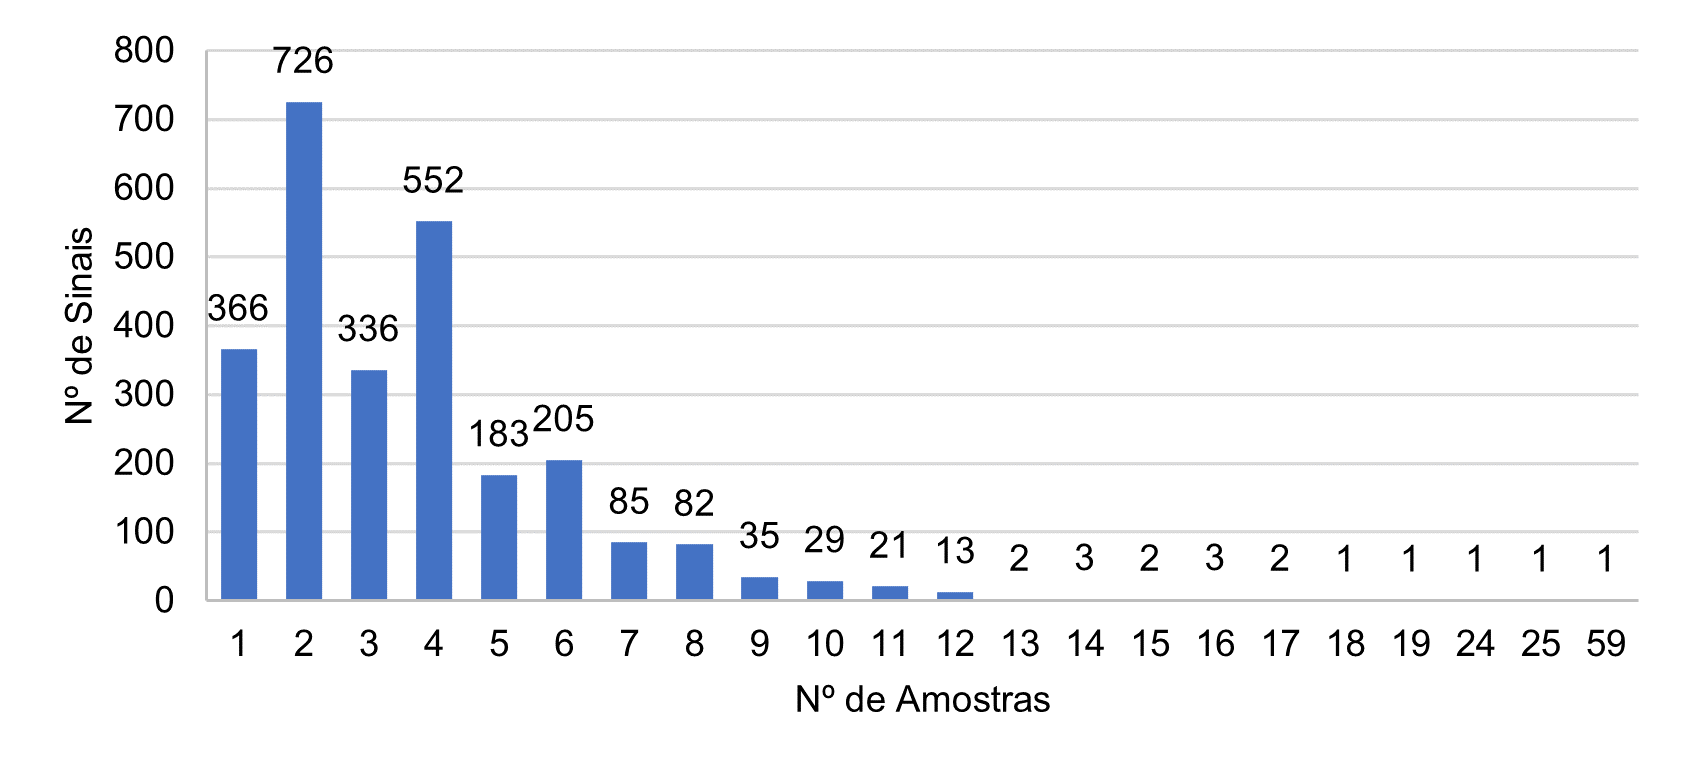
\includegraphics[height=6cm]{capitulos/metodologia/imagens/dataset_resampling_antes}
    }%
    \hspace{1cm}
    \subcaptionbox{\label{subfig:dataset-resampling-depois}}{
        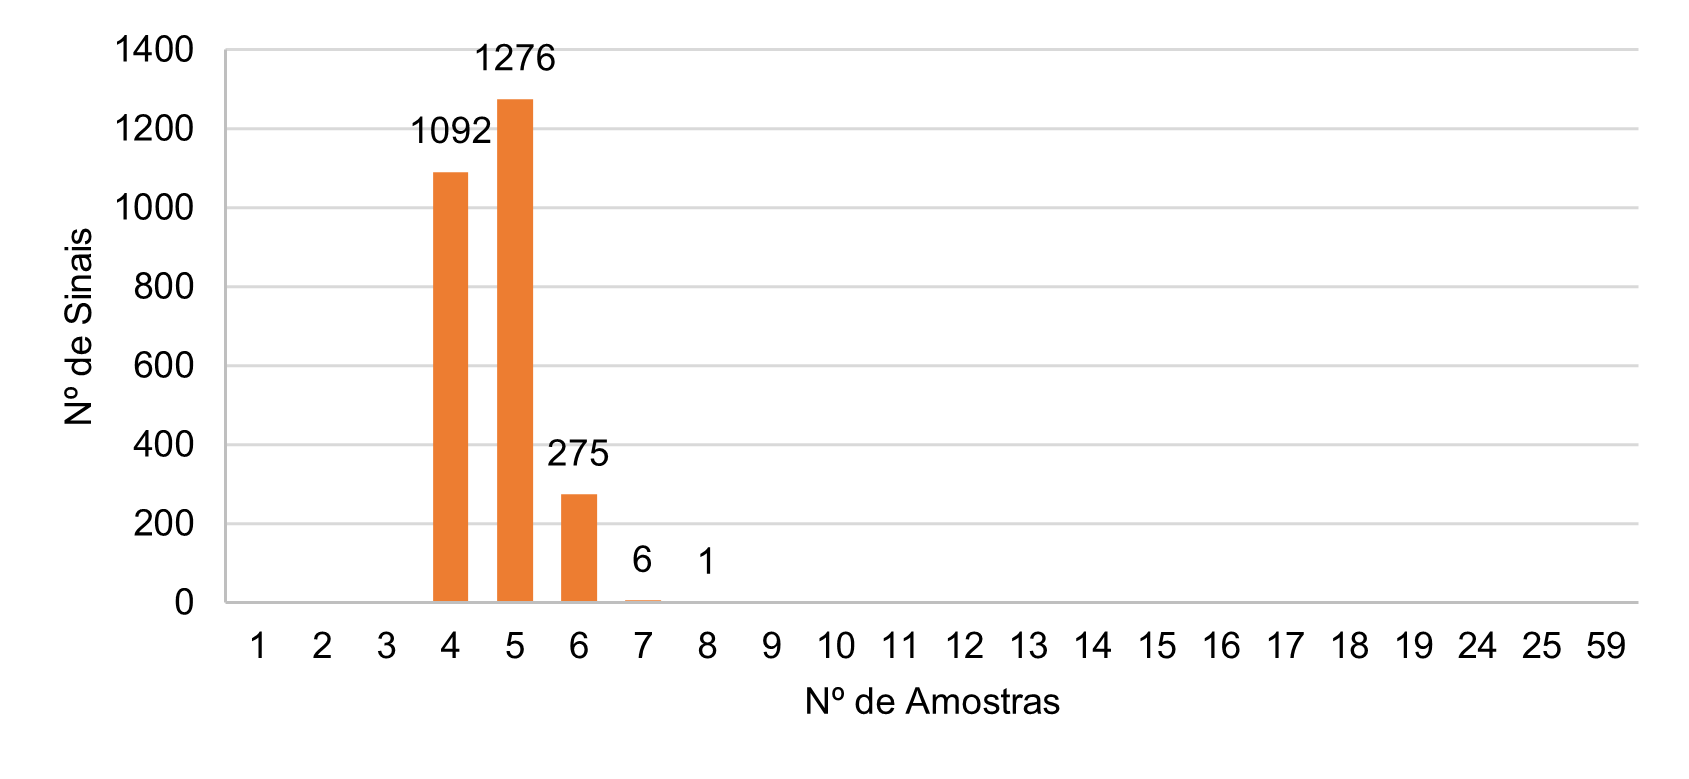
\includegraphics[height=6cm]{capitulos/metodologia/imagens/dataset_resampling_depois}
    }%
    \nomefonte{}
    \label{fig:dataset-resampling}
\end{figure}

Aplicamos então uma reamostragem \textit{naive random under-sampling} (ou sub-amostragem aleatória ingênua, que reduz o número de amostras através de uma seleção aleatória de algumas delas para os sinais que estão super-representados) seguida de uma \textit{naive random over-sampling} (ou sobre-amostragem aleatória ingênua, que replica aleatoriamente algumas das amostras existentes para os sinais que estão sub-representados).
Para estabelecer o novo número de amostras por sinal \(x'\), utilizamos a \autoref{eqn:resampling-target}: 

\begin{equation}
    \label{eqn:resampling-target}
    x' = round( \overline{a} + \ln(x) )
\end{equation}

Onde \(\overline{a}\) refere-se ao número médio de amostras por sinal no \textit{dataset} e \(x\) é o número de amostras para aquele sinal. Observe na \autoref{subfig:dataset-resampling-depois} como os dados ficaram organizados após a reamostragem. Em resumo, a equação faz com que o número de amostras por sinal se concentre mais uniformemente a partir do valor da média.



% SELEÇÃO DOS MODELOS -------------------------------------------

\subsection{Preparação dos modelos}
\label{sec:metodologia-reconhecimento-MODELOS}

% Com relação aos modelos utilizados para avaliar a eficácia da abordagem proposta ao reconhecer sinais, selecionamos três arquiteturas clássicas de modelos sequenciais -- que são LSTM \cite{hochreiter-1997-lstm}, GRU \cite{cho-2014-gru} e Transformer \cite{vaswani-2017-transformer} --, as quais nos ajudarão a estabelecer uma linha de base de referência. A partir do desempenho aferidos para essas arquiteturas, objetiva-se também prover clareza acerca de qual delas lida aborda melhor o problema em questão e é mais promissora para novas pesquisas nessa mesma linha.

Segundo \citeonline{jurafsky-2022-speech-lang-processing}, a linguagem é um fenômeno inerentemente temporal. Ela pode ser compreendida como uma sequência de eventos que se desdobram ao longo do tempo como um fluxo contínuo de dados. Arquiteturas sequenciais de aprendizagem profunda, por sua vez, são redes neurais projetadas para lidar diretamente com essa natureza sequencial, o que as torna capazes de capturar e explorar o aspecto temporal da língua.

Entre as mais populares dessas arquiteturas, estão a \acrfull{rnn} (e suas extensões, entre as quais o \acrfull{lstm} e a \acrfull{gru} são atualmente as principais) e o \textit{Transformer}. 

% Devido a isso, neste trabalho selecionamos algumas dessas arquiteturas para avaliar a eficácia da abordagem proposta, as quais são: \acrfull{lstm}~\cite{hochreiter-1997-lstm} e \acrfull{gru}~\cite{cho-2014-gru} -- que são extensões da arquitetura \acrfull{rnn}~\cite{mikolov-2010-rnn} -- e o \textit{Transformer}~\cite{vaswani-2017-transformer}. 

As \acrshortpl{rnn}~\cite{mikolov-2010-rnn} são redes que contêm ciclos (ou recorrências) em suas conexões, que fazem com que o valor de suas unidades sejam direta ou indiretamente dependentes de suas próprias saídas anteriores. 
Elas processam sequências de entrada uma palavra por vez, tentando prever a próxima palavra com base na atual e no contexto (ou estado oculto) anterior que, por sua vez, pode representar as informações de todas as palavras anteriores da sequência \cite{jurafsky-2022-speech-lang-processing}.
No entanto, \citeonline{lecun-2015-deep-learning,goodfellow-2016-deep-learning} afirmam que essas redes apresentam limitações em armazenar informações por um período muito longo de tempo -- dentre as quais estão os problemas de desaparecimento e explosão de gradiente --, o que demandou o desenvolvimento de extensões dessa arquitetura capazes de abordar melhor tais limitações.

% \citeonline{lecun-2015-deep-learning} afirmam que apesar do principal objetivo das \acrshortpl{rnn} ser aprender dependências de longo prazo, evidências teóricas e empíricas mostram que há desafios em aprender a armazenar informações por um tempo muito longo. Entre esses desafios estão os problemas de desaparecimento e explosão de gradientes, aos quais as \acrshortpl{rnn} estão passíveis. Devido a isso, várias extensões dessa arquitetura foram desenvolvidas no decorrer dos anos com o intuito de abordar melhor esses problemas.

O \acrshort{lstm}~\cite{hochreiter-1997-lstm} é a mais popular entre elas. Ele é capaz de aprender a gerenciar o contexto por conta própria, adicionando informação necessária e removendo aquela que não é mais, sem exigir que uma estratégia para isso seja codificada em sua arquitetura. Para isso, é utilizada uma camada específica para representar o contexto e um conjunto de portas, as quais controlam o fluxo de informações para dentro e para fora de suas células \cite{jurafsky-2022-speech-lang-processing}.
Segundo \citeonline{goodfellow-2016-deep-learning,lecun-2015-deep-learning}, essas redes são extremamente bem-sucedidas em diferentes aplicações, como reconhecimento de caligrafia, reconhecimento de fala, geração de caligrafia, tradução automática, legendagem de imagens e análise sintática.

%O \acrshort{lstm} é a mais popular delas e divide o gerenciamento do contexto em duas partes: na primeira, está a adição de informação que provavelmente será necessária para tomada de decisão posterior ao contexto; na segunda, está a remoção de informação que não é mais necessária. Com isso, o \acrshort{lstm} é capaz de aprender como gerenciar esse contexto e lidar com ambas as partes, e não exige que uma estratégia para isso seja codificada na arquitetura.
%Isso é feito utilizando-se uma camada explícita para representar o contexto e também unidades neurais especializadas que utilizam três portas (\textit{update gate}, \textit{forget gate} e \textit{output gate}) para controlar o fluxo de informações para dentro e para fora das unidades que compõem as camadas da rede neural. Essas portas, por sua vez, são implementadas como pesos adicionais que são ajustados durante o processo de treinamento e operam sequencialmente na entrada, na camada oculta e nas camadas de contexto anteriores \cite{jurafsky-2022-speech-lang-processing}.

% \citeonline{goodfellow-2016-deep-learning,lecun-2015-deep-learning} ressaltam que as redes \acrshort{lstm} mostraram ser extremamente bem-sucedidas em diferentes tipos de aplicações, como reconhecimento de caligrafia, reconhecimento de fala, geração de caligrafia, tradução automática, legendagem de imagens e análise sintática.

A \acrshort{gru}~\cite{cho-2014-gru}, por sua vez, é uma evolução do \acrshort{lstm}. De acordo com \citeonline{goodfellow-2016-deep-learning}, a principal diferença está na forma como elas controlam o fluxo de informações entre suas camadas: enquanto o \acrshort{lstm} adota três portas em suas células internas para isso (\textit{update gate}, \textit{forget gate} e \textit{output gate}), o \acrshort{gru} propõe uma simplificação das células e utiliza apenas duas portas (\textit{update gate} e \textit{reset gate}) \cite{ravanelli-2018-li-gru,goodfellow-2016-deep-learning}.

% A arquitetura \acrshort{gru} surgiu com o objetivo de simplificar o desenho das unidades internas do \acrshort{lstm} e, devido a isso, é considerada uma evolução desta. Segundo \citeonline{goodfellow-2016-deep-learning}, a principal diferença entre elas está na forma como elas controlam o fluxo de informação entre suas camadas. Enquanto que nas unidades do \acrshort{lstm} são utilizadas três portas para controlar a atualização, esquecimento e a saída de informação, no \acrshort{gru} uma única porta realiza o controle simultâneo do fator de esquecimento e da atualização do estado da unidade -- o que faz com que ela apresentem um total duas portas (denominadas \textit{update gate} e \textit{reset gate}) \cite{ravanelli-2018-li-gru,goodfellow-2016-deep-learning}.


Por outro lado, o \textit{Transformer}~\cite{vaswani-2017-transformer} é uma arquitetura que não é recorrente -- ao invés disso, baseia-se inteiramente num mecanismo de \textit{attention} (ou atenção) para estabelecer dependências globais entre os dados de entrada e saída. 
Ele é composta por blocos empilhados de redes multicamadas, as quais combinam camadas lineares simples, redes \textit{feed-forward} e camadas de \textit{self-attention} (ou auto-atenção) -- que, por sua vez, é a principal inovação desse tipo de arquitetura.
\citeonline{wolf-2020-transformers} afirmam que o \textit{Transformer} tornou-se rapidamente a arquitetura dominante para o \acrshort{nlp} e tem superado modelos alternativos como \acrshortpl{cnn} e \acrshortpl{rnn} sobretudo em tarefas de compreensão e geração de linguagem natural. Além disso, sua arquitetura escalável facilita o treinamento paralelo eficiente e a captura do contexto de sequências muito longas 
\cite{vaswani-2017-transformer,jurafsky-2022-speech-lang-processing,wolf-2020-transformers}.


% TODO: falar de encoder-decoder?

Tarefas de \acrfull{mt} utilizam um tipo de arquitetura conhecido como \textit{Encoder-Decoder} ou \textit{Sequence-to-Sequence} \cite{cho-2014-encoder-decoder,sutskever-2014-seq-to-seq}





% This chapter introduces two important deep learning architectures designed to address these challenges: recurrent neural networks and transformer networks. Both approaches have mechanisms to deal directly with the sequential nature of language that allow them to capture and exploit the temporal nature of language. The recurrent network offers a new way to represent the prior context, allowing the model’s decision to depend on information from hundreds of words in the past. The transformer offers new mechanisms (self-attention and positional encodings) that help represent time and help focus on how words relate to each other over long distances.


% LSTM
% LSTM networks have been shown to learn long-term dependencies more easilythan the simple recurrent architectures, first on artificial datasets designed fortesting the ability to learn long-term dependencies (Bengio et al., 1994; Hochreiterand Schmidhuber, 1997; Hochreiter et al., 2001), then on challenging sequenceprocessing tasks where state-of-the-art performance was obtained (Graves, 2012;Graves et al., 2013; Sutskever et al., 2014). Variants and alternatives to the LSTMthat have been studied and used are discussed next.
% The LSTM has been found extremely successfulin many applications, such as unconstrained handwriting recognition (Graveset al., 2009), speech recognition (Graves et al., 2013; Graves and Jaitly, 2014),handwriting generation (Graves, 2013), machine translation (Sutskever et al., 2014),image captioning (Kiros et al., 2014b; Vinyals et al., 2014b; Xu et al., 2015), andparsing (Vinyals et al., 2014a).
% \cite{goodfellow-2016-deep-learning}


% GRU
% Which pieces of the LSTM architecture are actually necessary? What other successful architectures could be designed that allow the network to dynamicallycontrol the time scale and forgetting behavior of different units? Some answers to these questions are given with the recent work on gated RNNs, whose units are also known as gated recurrent units, or GRUs (Cho et al., 2014b;Chung et al., 2014, 2015a; Jozefowicz et al., 2015; Chrupala et al., 2015).
% \cite{goodfellow-2016-deep-learning}

% The main difference with the LSTM is that a single gating unit simultaneously controls the forgetting factor and the decision to update the state unit.
% \cite{goodfellow-2016-deep-learning}

% This evolution has recently led to a novel architecture called Gated Recurrent Unit (GRU) [8], that simplifies the complex LSTM cell design.
% [...]
% A noteworthy attempt to simplify LSTMs has recently led to a novel model called Gated Recurrent Unit (GRU) [8], [47], that is based on just two multiplicative gates.
% \cite{ravanelli-2018-li-gru}


% TRANSFORMER
% \cite{jurafsky-2022-speech-lang-processing}
% transformers – an approach to sequence processing that eliminates recurrent connections and returns to architectures reminiscent of the fully connected networks described earlier in Chapter 7.
% Transformers map sequences of input vectors (x1; :::;xn) to sequences of output vectors (y1; :::;yn) of the same length. 
% Transformers are made up of stacks of transformer blocks, which are multilayer networks made by combining simple linear layers, feedforward networks, and self-attention layers, the key innovation of transformers. Self-attention allows a network to directly extract and use information from arbitrarily large contexts without the need to pass it through intermediate recurrent connections as in RNNs. We’ll start by describing how self-attention works and then return to how it fits into larger transformer blocks.


% \cite{vaswani-2017-transformer}
% In this work we propose the Transformer, a model architecture eschewing recurrence and instead relying entirely on an attention mechanism to draw global dependencies between input and output. The Transformer allows for significantly more parallelization and can reach a new state of the art in translation quality after being trained for as little as twelve hours on eight P100 GPUs.


% \cite{wolf-2020-transformers}
% Transformer architectures have facilitated building higher-capacity models and pretraining has made it possible to effectively utilize this capacity for a wide variety of tasks.

% The Transformer (Vaswani et al., 2017) has rapidly become the dominant architecture for natural language processing, surpassing alternative neural models such as convolutional and recurrent neural networks in performance for tasks in both natural language understanding and natural language generation. The architecture scales with training data and model size, facilitates efficient parallel training, and captures long-range sequence features



% 10. MACHINE TRANSLATION AND ENCODER-DECODER MODELS
% \cite{jurafsky-2022-speech-lang-processing}

% This chapter introduces machine translation (MT), the use of computers to translate from one language to another.
% Of course translation, in its full generality, such as the translation of literature, or poetry, is a difficult, fascinating, and intensely human endeavor, as rich as any other area of human creativity.
% Machine translation in its present form therefore focuses on a number of very practical tasks. Perhaps the most common current use of machine translation is information for information access.

% Another common use of machine translation is to aid human translators. MT systems are routinely used to produce a draft translation that is fixed up in a post-editing phase by a human translator. This task is often called computer-aided translation or CAT. CAT is commonly used as part of localization: the task of adapting content or a product to a particular language community.

% Finally, a more recent application of MT is to in-the-moment human communication needs. This includes incremental translation, translating speech on-the-fly before the entire sentence is complete, as is commonly used in simultaneous interpretation. Image-centric translation can be used for example to use OCR of the text on a phone camera image as input to an MT system to translate menus or street signs.

% The standard algorithm for MT is the encoder-decoder network, also called the sequence to sequence network, an architecture that can be implemented with RNNs or with Transformers. We’ve seen in prior chapters that RNN or Transformer architecture can be used to do classification (for example to map a sentence to a positive or negative sentiment tag for sentiment analysis), or can be used to do sequence labeling (for example to assign each word in an input sentence with a part-of-speech, or with a named entity tag). For part-of-speech tagging, recall that the output tag is associated directly with each input word, and so we can just model the tag as output yt for each input word xt .
% Encoder-decoder or sequence-to-sequence models are used for a different kind of sequence modeling in which the output sequence is a complex function of the entire input sequencer; we must map from a sequence of input words or tokens to a sequence of tags that are not merely direct mappings from individual words. 
% Machine translation is exactly such a task: the words of the target language don’t necessarily agree with the words of the source language in number or order.
% [...]
% Encoder-decoder networks are very successful at handling these sorts of complicated cases of sequence mappings. Indeed, the encoder-decoder algorithm is not just for MT; it’s the state of the art for many other tasks where complex mappings between two sequences are involved. These include summarization (where we map from a long text to its summary, like a title or an abstract), dialogue (where we map from what the user said to what our dialogue system should respond), semantic parsing (where we map from a string of words to a semantic representation like logic or SQL), and many others.

% 10.2 The Encoder-Decoder Model
% Encoder-decoder networks, or sequence-to-sequence networks, are models capable of generating contextually appropriate, arbitrary length, output sequences. Encoder-decoder networks have been applied to a very wide range of applications including machine translation, summarization, question answering, and dialogue.
% The key idea underlying these networks is the use of an encoder network that takes an input sequence and creates a contextualized representation of it, often called the context. This representation is then passed to a decoder which generates a task specific output sequence. Fig. 10.3 illustrates the architecture
% [FIGURE]

% Encoder-decoder networks consist of three components:
% 1. An encoder that accepts an input sequence, xn1, and generates a corresponding sequence of contextualized representations, hn1. LSTMs, convolutional networks, and Transformers can all be employed as encoders.
% 2. A context vector, c, which is a function of hn1, and conveys the essence of the input to the decoder.
% 3. A decoder, which accepts c as input and generates an arbitrary length sequence of hidden states hm1, from which a corresponding sequence of output states ym1, can be obtained. Just as with encoders, decoders can be realized by any kind of sequence architecture.

% 10.3 Encoder-Decoder with RNNs
% [...]

% 10.4 Attention
% The simplicity of the encoder-decoder model is its clean separation of the encoder—
% which builds a representation of the source text—from the decoder, which uses this
% context to generate a target text. In the model as we’ve described it so far, this
% context vector is hn, the hidden state of the last (nth) time step of the source text.
% This final hidden state is thus acting as a bottleneck: it must represent absolutely
% everything about the meaning of the source text, since the only thing the decoder
% knows about the source text is what’s in this context vector (Fig. 10.8). Information
% at the beginning of the sentence, especially for long sentences, may not be equally
% well represented in the context vector.
% The attention mechanism is a solution to the bottleneck problem, a way of
% allowing the decoder to get information from all the hidden states of the encoder,
% not just the last hidden state.

% The idea of attention is instead to create the single fixed-length vector c by taking
% a weighted sum of all the encoder hidden states. The weights focus on (‘attend
% to’) a particular part of the source text that is relevant for the token the decoder is
% currently producing. Attention thus replaces the static context vector with one that
% is dynamically derived from the encoder hidden states, different for each token in
% decoding.
% [...]
% The weights Ws, which are then trained during normal end-to-end training, give the
% network the ability to learn which aspects of similarity between the decoder and
% encoder states are important to the current application. This bilinear model also
% allows the encoder and decoder to use different dimensional vectors, whereas the
% simple dot-product attention requires that the encoder and decoder hidden states
% have the same dimensionality.

% 10.5 Beam Search
% [...]

% 10.6 Encoder-Decoder with Transformers
% The encoder-decoder architecture can also be implemented using transformers (rather
% than RNN/LSTMs) as the component modules. At a high-level, the architecture,
% sketched in Fig. 10.15, is quite similar to what we saw for RNNs. It consists of an
% encoder that takes the source language input words X = x1; :::;xT and maps them
% to an output representation Henc = h1; :::;hT ; usually via N = 6 stacked encoder
% blocks. The decoder, just like the encoder-decoder RNN, is essentially a conditional
% language model that attends to the encoder representation and generates the target
% words one by one, at each timestep conditioning on the source sentence and the
% previously generated target language words.
% [IMAGE]
% But the components of the architecture differ somewhat from the RNN and also
% from the transformer block we’ve seen. First, in order to attend to the source language,
% the transformer blocks in the decoder has an extra cross-attention layer.
% Recall that the transformer block of Chapter 9 consists of a self-attention layer that
% attends to the input from the previous layer, followed by layer norm, a feed forward
% layer, and another layer norm. The decoder transformer block includes an
% extra layer with a special kind of attention, cross-attention (also sometimes called
% encoder-decoder attention or source attention). Cross-attention has the same form
% as the multi-headed self-attention in a normal transformer block, except that while
% the queries as usual come from the previous layer of the decoder, the keys and values
% come from the output of the encoder.




% \cite{goodfellow-2016-deep-learning}
% https://www.deeplearningbook.org/contents/rnn.html

% 10.4 Encoder-Decoder Sequence-to-Sequence Architectures
% Here we discuss how an RNN can be trained to map an input sequence to anoutput sequence which is not necessarily of the same length. This comes up inmany applications, such as speech recognition, machine translation and questionanswering, where the input and output sequences in the training set are generallynot of the same length (although their lengths might be related).
% [IMAGE]
% The simplest RNN architecture for mapping a variable-length sequence toanother variable-length sequence was first proposed by Cho et al. (2014a) [https://aclanthology.org/D14-1179/] and shortly after by Sutskever et al. (2014) [https://arxiv.org/abs/1409.3215], who independently developed that architecture and were the first to obtain state-of-the-art translation using this approach.

% The former system is based on scoring proposals generated by another machinetranslation system, while the latter uses a standalone recurrent network to generatethe translations. These authors respectively called this architecture, illustratedin figure 10.12, the encoder-decoder or sequence-to-sequence architecture. Theidea is very simple: (1) AnencoderorreaderorinputRNN processes the inputsequence. The encoder emits the contextC, usually as a simple function of itsfinal hidden state. (2) AdecoderorwriteroroutputRNN is conditioned onthat fixed-length vector (just as in figure 10.9) to generate the output sequenceY= (y(1), . . . , y(ny)). 

% One clear limitation of this architecture is when the contextCoutput by theencoder RNN has a dimension that is too small to properly summarize a longsequence. This phenomenon was observed by Bahdanau et al. (2015) in the contextof machine translation. They proposed to makeCa variable-length sequence ratherthan a fixed-size vector. Additionally, they introduced anattention mechanismthat learns to associate elements of the sequenceCto elements of the outputsequence. See section 12.4.5.1 for more details.







% \cite{jurafsky-2022-speech-lang-processing}
% The most commonly used such extension to RNNs is the Long short-term
% memory (LSTM) network (Hochreiter and Schmidhuber, 1997). LSTMs divide the context management problem into two sub-problems: removing information no longer needed from the context, and adding information likely to be needed for later decision making. The key to solving both problems is to learn how to manage this context rather than hard-coding a strategy into the architecture. LSTMs accomplish this by first adding an explicit context layer to the architecture (in addition to the usual recurrent hidden layer), and through the use of specialized neural units that make use of gates to control the flow of information into and out of the units that comprise the network layers. These gates are implemented through the use of additional weights that operate sequentially on the input, and previous hidden layer, and previous context layers.
% The gates in an LSTM share a common design pattern; each consists of a feedforward layer, followed by a sigmoid activation function, followed by a pointwise multiplication with the layer being gated. The choice of the sigmoid as the activation function arises from its tendency to push its outputs to either 0 or 1. Combining this with a pointwise multiplication has an effect similar to that of a binary mask. Values in the layer being gated that align with values near 1 in the mask are passed through nearly unchanged; values corresponding to lower values are essentially erased.



% ======================================
% \cite{goodfellow-2016-deep-learning}
% 
% Chapter 10
% https://www.deeplearningbook.org/contents/rnn.html
%
% 10.10 The Long Short-Term Memory and Other GatedRNNs (pg 404)
% As of this writing, the most effective sequence models used in practical applications are called gated RNNs. These include the long short-term memory and networks based on the gated recurrent unit.
% Like leaky units, gated RNNs are based on the idea of creating paths through time that have derivatives that neither vanish nor explode. Leaky units did this with connection weights that were either manually chosen constants or were parameters. Gated RNNs generalize this to connection weights that may change at each time step.
% Leaky units allow the network to accumulate information (such as evidence fora particular feature or category) over a long duration. Once that information has been used, however, it might be useful for the neural network to forget the old state. For example, if a sequence is made of subsequences and we want a leaky unit to accumulate evidence inside each sub-subsequence, we need a mechanism to forget the old state by setting it to zero. Instead of manually deciding when to clear the state, we want the neural network to learn to decide when to do it. This is what gated RNNs do.

% 10.10.1 LSTM
% The clever idea of introducing self-loops to produce paths where the gradientcan flow for long durations is a core contribution of the initiallong short-termmemory(LSTM) model (Hochreiter and Schmidhuber, 1997). A crucial additionhas been to make the weight on this self-loop conditioned on the context, rather thanfixed (Gers et al., 2000). By making the weight of this self-loop gated (controlledby another hidden unit), the time scale of integration can be changed dynamically.In this case, we mean that even for an LSTM with fixed parameters, the time scaleof integration can change based on the input sequence, because the time constantsare output by the model itself. 
% The LSTM has been found extremely successfulin many applications, such as unconstrained handwriting recognition (Graveset al., 2009), speech recognition (Graves et al., 2013; Graves and Jaitly, 2014),handwriting generation (Graves, 2013), machine translation (Sutskever et al., 2014),image captioning (Kiros et al., 2014b; Vinyals et al., 2014b; Xu et al., 2015), andparsing (Vinyals et al., 2014a).
% [...]
% Deeper architectures have also been successfully used (Graves et al.,2013; Pascanu et al., 2014a). Instead of a unit that simply applies an element-wisenonlinearity to the affine transformation of inputs and recurrent units, LSTMrecurrent networks have “LSTM cells” that have an internal recurrence (a self-loop),in addition to the outer recurrence of the RNN. Each cell has the same inputs andoutputs as an ordinary recurrent network, but also has more parameters and asystem of gating units that controls the flow of information.
% LSTM networks have been shown to learn long-term dependencies more easilythan the simple recurrent architectures, first on artificial datasets designed fortesting the ability to learn long-term dependencies (Bengio et al., 1994; Hochreiterand Schmidhuber, 1997; Hochreiter et al., 2001), then on challenging sequenceprocessing tasks where state-of-the-art performance was obtained (Graves, 2012;Graves et al., 2013; Sutskever et al., 2014). Variants and alternatives to the LSTMthat have been studied and used are discussed next.

% 10.10.2 Other Gated RNNs
% Which pieces of the LSTM architecture are actually necessary? What other successful architectures could be designed that allow the network to dynamically control the time scale and forgetting behavior of different units? Some answers to these questions are given with the recent work on gated RNNs,whose units are also known as gated recurrent units, or GRUs (Cho et al., 2014b;Chung et al., 2014, 2015a; Jozefowicz et al., 2015; Chrupala et al., 2015). The main difference with the LSTM is that a single gating unit simultaneously controls the forgetting factor and the decision to update the state unit.



% ================================
% \cite{lecun-2015-deep-learning}
% RNNs, once unfolded in time (Fig. 5), can be seen as very deep feedforward networks in which all the layers share the same weights. Although their main purpose is to learn long-term dependencies, theoretical and empirical evidence shows that it is difficult to learn to store information for very long78.
% To correct for that, one idea is to augment the network with an explicit memory. The first proposal of this kind is the long short-term memory (LSTM) networks that use special hidden units, the natural behaviour of which is to remember inputs for a long time79. A special unit called the memory cell acts like an accumulator or a gated leaky neuron: it has a connection to itself at the next time step that has a weight of one, so it copies its own real-valued state and accumulates the external signal, but this self-connection is multiplicatively gated by another unit that learns to decide when to clear the content of the memory.
% LSTM networks have subsequently proved to be more effective than conventional RNNs, especially when they have several layers for each time step87, enabling an entire speech recognition system that goes all the way from acoustics to the sequence of characters in the transcription. LSTM networks or related forms of gated units are also currently used for the encoder and decoder networks that perform so well at machine translation17,72,76
